\documentclass[11pt,a4paper]{report}

\usepackage{url}
\usepackage{graphicx}
\usepackage[all]{xy}
\usepackage{amsmath}
\usepackage{amsthm}
\usepackage{amsfonts}
\usepackage{todonotes}
\usepackage{array}
\usepackage{listings}
\usepackage{xcolor}
\usepackage[a4paper]{geometry}

\usepackage{hyperref}
\usepackage{subcaption}
\usepackage{ dsfont }
\usepackage{algorithm}
\usepackage{algpseudocode}


\newtheorem{definition}{Definition}
\DeclareMathOperator*{\argmax}{arg\,max}

\makeatletter %otherwise geometry resets everything

\renewcommand\paragraph{\@startsection{paragraph}{4}{\z@}%
            {-2.5ex\@plus -1ex \@minus -.25ex}%
            {1.25ex \@plus .25ex}%
            {\normalfont\normalsize\bfseries}}
\makeatother
\setcounter{secnumdepth}{4} % how many sectioning levels to assign numbers to
\setcounter{tocdepth}{4}    % how many sectioning levels to show in ToC

\makeatother

\setlength{\itemsep}{0cm}
\setlength{\voffset}{0cm}
\setlength{\headheight}{0cm}
\setlength{\topmargin}{0cm}
\setlength{\extrarowheight}{3pt} %for superscripts in tabular
\setlength{\arraycolsep}{4pt}
\lstset{basicstyle = \footnotesize, breaklines = true}

\graphicspath{{imgs/}}

\sloppy

\begin{document}
\begin{titlepage}
\begin{center}
\textsc{\LARGE Master thesis\\Computing Science}\\[1.5cm]

\includegraphics[height=100pt]{logo}

\vspace{0.4cm}
\textsc{\Large Radboud University}\\[1cm]
\hrule
\vspace{0.4cm}
\textbf{\huge Spatial state-space dimensionality reduction in model-free reinforcement learning}\\[0.4cm]
\hrule
\vspace{2cm}
\begin{minipage}[t]{0.45\textwidth}
\begin{flushleft} \large
\textit{Author:}\\
Niels van Velzen\\
s4269454
\end{flushleft}
\end{minipage}
\begin{minipage}[t]{0.45\textwidth}
\begin{flushright} \large
\textit{First supervisor/assessor:}\\
Dr., N. H. Jansen\\
\texttt{n.jansen@cs.ru.nl}\\[0.8cm]
\textit{Second supervisors:}\\
MSc., D. M. Gro{\ss}\\
\texttt{D.Gross@cs.ru.nl}\\[0.4cm]
MSc., C. Schmidl\\
\texttt{c.schmidl@cs.ru.nl}\\[0.8cm]
\textit{Second assessor:}\\
Dr., T. Kachman\\
\texttt{tal.kachman@donders.ru.nl}\\[1.0cm]
\end{flushright}
\end{minipage}
\vfill
{\large \today}
\end{center}
\end{titlepage}

\begin{abstract}
The abstract of your thesis is a brief description of the research hypothesis,
scientific context, motivation, and results.
The preferred size of an abstract is one paragraph or one page of text.
\end{abstract}


\tableofcontents

\chapter{Introduction}\label{introduction}
% - gebruik state-space dimensionality reduction stukje voor problem statement, icm dat methodes hiervoor mogelijk los van RL getraind kunnen worden en dus gebruikbaar zijn en kunnen leiden to mindere interactie met fysieke/real life environment + kunnen onnodige info of noise wegfilteren (zoals genoemd in related work)
\begin{itemize}
\item describe the problem / research question
\item motivate why this problem must be solved
\item demonstrate that a (new) solution is needed
\item explain the intuition behind your solution
\item motivate why / how your solution solves the problem (this is technical)
\item explain how it compares with related work
\end{itemize}
%

\chapter{Related Work}\label{relatedwork}
State-space dimensionality reduction has been a topic of interest in RL for several years. Curran et al. \cite{mario} used PCA to reduce the dimensionality of the state-space in a Super Mario environment. They found that with the right number of principal components, an agent using PCA was able to converge to a better policy and need less episodes than an agent using the full observation. Unlike the Starcraft II environment used in our research having image/grid based observations, their states and observations are comprised of non-spatial related variables; to, for instance, denote the presence of one or more enemies within one gridcell distance of Mario's position, they use one variable with $2^8$ possible values ($0-255$). Hence we are using PCA in a different setting, with an observation format more commonly used in modern RL. Furthermore they use the Q-learning algorithm (mentioned in section \ref{pl-dqn}) which is not a state-of-the-art learning algorithm anymore.

Research has also been done with regards to using autoencoders for state-space-dimensionality reduction in RL. Lange and Riedmiller in 2010 \cite{AE_2010} used visual data as observations and found that the agent was able to find an optimal policy using lower dimensional data from the autoencoder. They did not compare the performance of this agent with any other agent. Furthermore, their system only has $31$ possible states, which is very limited; in contrast, our environment has a total of $731.187$ possible states. 

In 2016, Van Hoof et al. \cite{AE_2016} used an autoencoder to project noisy sensor data unto a lower dimensional space. They found that the agent using the autoencoder was far better able to find a good policy than the agent using full observations. This was explained as the agent being too sensitive to noisy data, hence being unable to train even decently. Our research in contrast explores an environment where the baseline (i.e. vanilla) agent is able to train to a good policy.

In 2019, Prakash et al. \cite{AE_2019} also used an autoencoder on visual data to project the observation data onto a lower dimensional space. They found that an agent using the autoencoder far outperformed the baseline agent. Again though, the baseline agent did not find a decent policy, though the authors claim that with enough episodes it would have.

Another paper in 2019 by Gelada et al. \cite{deepmdp} compared using a DeepMDP with using an autoencoder for state-space dimensionality reduction. They found that in simpler environments a DeepMDP can find better representations on lower dimensionality space than an autoencoder. Simultaneously though, they also find that in more complex environments, like Atari games, DeepMDPs can have trouble finding a good representation and that its loss can be difficult to optimize. They also find that a DeepMDP agent generally outperforms a baseline (i.e. vanilla) agent. 

%TODO demonstrating that you have found a \emph{new} solution / approach / method?

\chapter{Preliminaries}\label{preliminaries}
To get a better understanding of our research, we provide some preliminary information in this section. We will start by introducing the concept of \emph{reinforcement learning} in section \ref{pl-rl}. Following this, we will discuss \emph{state-space dimensionality reduction}, including several methods to do this in section \ref{pl-dimensionality}.
 
\section{Reinforcement learning}\label{pl-rl}
The main theoretical framework we are working in, is called \emph{reinforcement learning} (RL). This is a form of \emph{machine learning}, the area of artificial intelligence that is concerned with creating computer programs that can solve problems by learning from data. The two other main forms of machine learning are \emph{supervised learning} and \emph{unsupervised  learning}. The distinct feature of RL is that it learns from feedback through trial and error \cite[p. 2-5]{grokking}.

We will now examine RL more closely and formally, as well as discuss \emph{neural networks} and a specific RL algorithm used in our research called \emph{DDQN}.

 
\subsection{General overview}
As mentioned, RL is the area of artificial intelligence where problems are solved through trial and error using feedback. An example is a robot learning to bring a given package to a given location. The portion of the code responsible for the decision making, i.e. choosing an action, is called the \emph{agent}. Besides an agent, there is also the \emph{environment}, which entails everything other than the agent. In our package delivery example this could for instance be the hardware of the robot, the package to be delivered, wind conditions, the road, and any obstacle.

The environment is encoded in a set of variables, where all possible values of these variables are called the \emph{state-space}. In our example, some of these variables are the coordinates of the location of the robot, wind speed and direction, and the coordinates for the location where the package needs to be delivered. A single instantiation of the state-space is a \emph{state}. 

To be able to make any informed decision, the agent will need some information with regards to the current state. The information about a state received by the agent, i.e. the variables making up the state-space, is called an \emph{observation}. This observation might be partial; the agent might not receive all information about a state. In our example, the agent might not have any information about an obstacle on the road that it hasn't sensed yet.

Using this information, the agent makes a decision  about which action to take. The total set of possible actions for all states is the \emph{action-space}. A lot of different algorithms exist with regards to decision making and learning how to make better decision. In section \ref{pl-dqn} we will discuss the learning algorithm we will use, called \emph{double deep-Q-network}. Depending on the current state and the action taken by the agent, the environment might go to a new, different state. This change is encoded by a \emph{transition function}; given a state and action pair it returns the next state. 

The current mapping in the agent between a given state and a distribution over possible actions is called its \emph{policy}. The better its policy, the better it is able to solve the problem. To be able to improve its policy, the agent needs information about how well it has been performing. This feedback is given in the form of \emph{rewards}: the environment sends positive or negative rewards to the agent, informing it about how well it has performed. In our package delivery example, the robot might get a $+1$ reward whenever it delivers a package.

This results in an interaction cycle between the agent and the environment, depicted in figure \ref{fig:rl_cycle}. It begins with the agent receiving an observation. Then, it chooses an action. This results in the environment transitioning into a new state (possibly the same state as before having taken the action). After this, the environment send a new observation along with a reward to the agent, and the the agent chooses a new action. This interaction stops once the problem has been solved, or when some other constraint has been violated (like a time limit, or the robot getting into an unwanted state like the robot crashing into an object). When the cycle stops, we have finished an \emph{episode}. After this, the environment can be reset to start a new episode. To get to a well performing policy, the agent often needs hundreds or thousands of episodes \cite[p. 6-10]{grokking}. 

\begin{figure}[h]
    \centering
    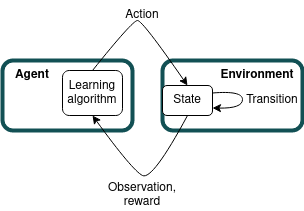
\includegraphics[width=0.5\textwidth]{rl-cycle}
    \caption{The cycle of interaction between the environment and an agent in reinforcement learning.}
    \label{fig:rl_cycle}
\end{figure}

Let us now formally define the reinforcement learning paradigm. RL problems are commonly modeled as \emph{Markov decision processes} (MDPs). 

\begin{definition} A Markov decision process (MDP) is a tuple $(S, A, T, R, S_{\theta})$, with state-space $S$, the action-space $A$, transition  probability function $T$: $S \rightarrow 2^{A \times Distr(S)}$ (thus modeling stochasticity), reward function $R$: $S \times A \times S \rightarrow \mathbb{R}$ and initial states distribution $S_{\theta}$. $T$ also describes the probability distribution for transitions, $p(s'|s,a)$: the probability of a transitioning to state $s'$ given state-action pair $(s, a)$ \cite[p. 45-62]{grokking}.
\end{definition}

A graphical example of an MDP can be seen in figure \ref{fig:mdp}.

\begin{figure}[h]
    \centering
    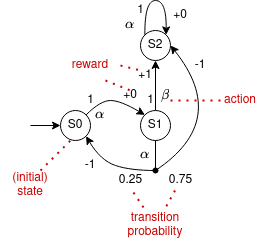
\includegraphics[width=0.5\textwidth]{MDP}
    \caption{Example of a Markov decision process (MDP).}
    \label{fig:mdp}
\end{figure}

The reward function models the expected reward for a transition; given a transition consisting of a state, action and next state, it returns the expected reward.

The reward function is defined as function $r$:
\begin{equation}
	\label{reward}
	r(s, a, s') = \mathds{E}[R_{t} | S_{t-1} = s, A_{t-1} = a, S_{t} = s']
\end{equation}
where $t$ is the timestep and $R_{t} \in R \subset \mathbb{R}$ \cite[p. 54]{grokking}.

To get to its best possible policy, an agent tries to maximize its total sum of expected reward. This is also known as the \emph{return} $G$: 
\begin{equation}
G_t = R_{t+1} + \gamma G_{t+1}
\end{equation}
with timestep $t$ and a discount factor $\gamma \in [0,1]$ to set the weight of future rewards \cite[p. 67]{grokking}. 

Often, an agent does not know the underlying MDP to a problem. Therefore, we must use a way without using the underlying MDP to find the best possible policy (i.e. the policy giving the highest expected return). To evaluate any policy ${\pi}$ and be able to compare its performance to other policies, we can use the \emph{Bellman equation}. This tells us what the expected return is when starting at any state $s$, following policy $\pi$. This is known as the \emph{state-value function} (V-function, or $V^{\pi}(s)$).
\begin{equation}
v_\pi (s) = \sum_{a} \pi (a|s) \sum_{s', r} p(s', r|s,a)[r + \gamma v_\pi (s')], \forall s \in S
\end{equation} 

For any state, we look at all possible actions. For each resulting state-action pair, we look at all possible transitions and sum the corresponding reward with the value of the next state weighted by the discount factor $\gamma$. This sum is then weighted by the probability of this transition. The resulting value is summed for all possible transitions of this state-action pair, and we then sum these results for all actions of the given state. This results in the value for this state \cite[p. 73]{grokking}.

Having a method of finding the value of a state, is the first step towards an agent being able to figure out the best possible policy. When an agent tries to improve its policy, it can make use of the \emph{action-value function} (Q-function, or $Q^\pi (s, a)$. This tells us the expectation of returns following policy $\pi$ after having taken action $a$ in state $s$. It is defined as follows:

\begin{equation}
q_\pi (s,a) = \sum_{s', r} p(s', r|s,a)[r + \gamma v_\pi (s')], \forall s \in S, \forall a \in A(s)
\end{equation}
For all possible state-action pairs $(s,a)$, we calculate their value by looking at all their possible transitions, taking the corresponding reward, sum this by the state-value of the next state weighted by the discount factor $\gamma$, and weigh this sum with the probability of this transition happening \cite[p. 74]{grokking}.

An agent is in search of an optimal policy: a policy that has an expected return greater or equal to all other possible policies. Such a policy has the optimal action-value function, known as the $q*$ function: this is the action-value function with the highest value over all possible policies. Therefore, if the agent is able to figure out the $q*$ function, it knows the optimal action for each state and thus the optimal policy. Approximating this $q*$ is the approach for most current state-of-the-art learning algorithms, including the one used in this research: double deep-Q-network (DDQN). 

We will explain how DDQN is able to approximate the $q*$ function in section \ref{pl-dqn}. However, to understand DDQN, we will first need to introduce \emph{neural networks}. This is because in order to approximate the $q*$ function, an agent will need to keep track of the action-value for all state-action pairs. Storing these values in a table is not scalable: for problems with large (or continuous) state-spaces and large action-spaces, the table would be became way too large to be able to work with. Therefore, we need a way to approximate this table, which is what neural networks are used for. We will now first explore neural networks, before explaining DDQN.

\subsection{Artificial neural networks}\label{pl-nn}
The use of artificial neural networks (ANN) in reinforcement learning, is known as \emph{deep RL} \cite[p. 5]{grokking}. ANNs are a way of being able to use RL in problems with large state-space and large action-spaces. This is because ANNs are able to approximate both linear and non-linear functions in an efficient way\cite[p. 165-166]{nn}. Therefore, they can be used to approximate the $q*$, instead of using an action-value table to know the $q*$ function. We will now shortly examine ANNs, using \cite[p. 164-366]{nn}.

ANNs consist of artificial neurons: a mathematical function that sums its input which is used to produce an output. These neurons are grouped into different layers, consisting of any number of neurons. Firstly, there is the input layer. In the case of RL, its input is most often the variables making up an observation. Secondly, there is the output layer, creating the output of the network. In between these two layers there usually are other layers. These are known as the hidden layers. 

To produce an output, a neuron sums its input. Each input of a neuron has its own weight: a variable settings its importance. The network learns to produce better output by changing these weights. After summing the weighted inputs, the result is passed through an (often nonlinear) activation function. This produces the output of the neuron. 

Different types of neural networks exist. One important difference here is the connections between neurons. The simplest form is a \emph{feedforward} neural network. Here, each neuron is only connected to neurons of the next layer, meaning there are no cycles. They are often fully connected: a neuron passes its output to each neuron of the next layer. An example of fully connected feedforward neural network can be seen in figure \ref{fig:nn}.

Another important type of neural network is a \emph{convolutional neural network} (CNN). This is a network that is useful for grid-like data, like image data. It is well suited for applications like image recognition. Such a network makes use of at least one convolutional layer. A convolutional layer consists of multiple kernels (or: filters): a set of learnable parameters. Each kernel convolves across the input to produce a feature map (or: activation map). Since each kernel has different parameters, each feature map will highlight different features of the input. These feature maps are then stacked to produce the output of the convolutional layer.

To improve the given output, a network can update its weights. For this it needs a loss function that computes how incorrect given output was. To calculate how much each weight needs to be changed, backpropagation is used. This computes the gradient for each weight with respect to the loss function. This way, loss can be minimized out therefore the output optimized.

\begin{figure}[h]
    \centering
    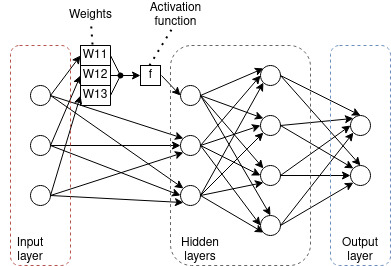
\includegraphics[width=0.5\textwidth]{nn}
    \caption{Example of a fully connected feedforward artificial neural network. For one node, example weights and activation function are shown.}
    \label{fig:nn}
\end{figure}

For more details on artificial neural networks, we refer to \cite{nn}. ANNs are a central part of the learning algorithm used in this paper: double deep-Q-network, which we will now examine.

\subsection{Double deep-q-network}\label{pl-dqn}
Before going into the learning algorithm DDQN, it is useful to start by looking at other algorithms preceding DDQN. Firstly we will look at \emph{Q-learning} and \emph{deep-Q-learning} (DQN). 

The RL approach taken in Q-learning is arguably the most used approach in RL \cite{qlearning}. It uses a table, the Q-table, to keep track of the Q-function determining the agent's policy. This Q-table is updated with new information gathered by the agent, to ultimately find an optimal policy by approximating $Q*$.

This is done through a cycle of interactions of the agent with the environment. The agent starts by getting an observation and choosing an action. The environment moves to a new state and the agent receives a new observation and a reward for the current transition. Then the Q-table is updated and the cycle starts over until we reach the end of our episode. Depending on the problem, the agent will need hundreds or thousands of episodes to get the Q-table to approximate the $Q*$ function.

When choosing an action, exploitation needs to be balanced with exploration. The agent needs to explore different actions in the same state to find out what happens and explore as many states as possible. Simultaneously, the agent will only start performing well once it starts exploiting the updated Q-table. To do this, an \emph{$\epsilon$-greedy strategy} is used. Each time an action must be taken, the agent gets a random number between $0$ and $1$. Whenever this is lower than or equal to the hyperparameter $\epsilon$, a random action is taken, otherwise it takes chooses an action greedily based on the Q-table. In this strategy, $\epsilon$ is usually decayed over time, to slowly put more emphasis on exploitation.

To update the Q-table after a transition, the old Q-value is added to the new information gotten from this transition, known as the \emph{temporal difference}. The temporal difference is first weighted by a hyperparameter called the \emph{learning rate}. This temporal difference is the difference between the current estimate in the Q-table and the \emph{TD-target}, which is the Q-value we are now moving towards. Thus, it represents the error between the current Q-value and the new estimate and is therefore known as the \emph{TD-error}.

\begin{equation}
Q(s_t,a_t) \leftarrow Q(s_t,a_t) + \alpha \cdot (r_t + \gamma \cdot \max _{a} Q(s_{t+1},a) - Q(s_t,a_t))
\end{equation}

In this equation, $r_t$ is the reward for this transition, $\alpha$ the learning rate and $\gamma$ the discount factor. The TD-target is calculated by adding the reward to the maximum Q-value of the next state weighted by the discount factor. Subtracting the old Q-value from the TD-target gives the TD-error. 

As mentioned in section \ref{pl-rl}, the use of a Q-table is not scalable. Therefore, new algorithms were introduced that use neural networks. One such algorithm is DQN. DQN was first introduced in 2015 by V. Mnih, K. Kavukcuoglu and D. Silver, and was the first algorithm to apply RL to high dimensional data while getting human-level scores for Atari-games \cite{dqn}.

Instead of computing Q-values directly using a Q-table, DQN \emph{approximates} the Q-function using neural networks. Such a network takes as input a state observation, and produces as output the Q-value for all possible actions in this state. To act greedily, the agent must simply pick the action with the highest value in the output of the network.

To get the Q-values for a state, we pass the state to its policy network. This is the network representing the policy of the agent. To be able to compute the TD-error, we also pass the next state to a network, to get the max Q-value of the next state. However, we use a second network for this. If we were to use the same network, the target would change every time the policy network is updated, thereby having it chase its own tail. Having a second network, the target network, allows us to freeze targets for a certain number of steps (a hyperparameter), before updating the target network to equal the policy network.

Additionally, we don't train the policy network with every step, but use a hyperparameter to set how often we train the network. Thus, we must store \emph{experiences}: tuples containing information about a transition, including the initial state, next state, reward and whether we ended in a terminal state. When training the network, we train it on batches of these experiences, known as \emph{replay memory}. 

Thus, when training the policy network we pass batches of next states to the policy network to get their maximum Q-values. The corresponding rewards are added to calculate the TD-target. Then the initial states are passed to the policy network to get their Q-values. These values are then used to calculate the TD-error which used to calculate the loss using the loss-function. Then the policy network is updated by backpropagating the loss.

Now we can look at the algorithm used in this paper: double-DQN (DDQN). DDQN is every similar to DQN. The difference is in how the policy network is trained \cite{ddqn}. In DQN we are taking the maximum of all Q-values. Since these values are estimates that differ from their true value, DQN tends to overestimate the highest Q-value. Doing this often will lead to divergence \cite[p. 293-297]{grokking}. Implicitly we are using the target network for two things: to get the action with the highest value, and what its value is. To solve the problem of overestimating Q-values, DDQN separates these two concerns: we use the policy network to get the action with the highest Q-value and then use the target network to get this action's Q-value. This way, the target network cross-validates the estimates of the policy network.

The pseudocode for DDQN is given in figure \ref{alg:ddqn}. This shows its training step for optimizing the policy network. This method is called within the interaction between agent and environment as explained in section \ref{pl-rl}. In short, the agent will receive an observation from the environment and the agent will, in our case, use a {$\epsilon$}-greedy strategy to choose an action, where the policy network is used. Then, the environment transitions and gives a new observation to the agent. Hyperparameters are used to set the number of such steps in between training the policy network, and to set the number of steps between updating the target network.

\begin{algorithm}
\caption{DDQN training step \cite[p.299]{grokking}.}
\label{alg:ddqn}
\begin{algorithmic}
\State Sample $experiences$ from replay buffer
\State $states$, $actions$, $rewards$, $next\_states$, $terminals$ $\gets$ $experiences$
\State $indices\_a\_q\_sp$ $\gets$ $\argmax_a policy\_ network(next\_states)$
\State $q\_sp$ $\gets$ $target\_network(next\_states)$
\State $max\_a\_q\_sp$ $\gets$ $q\_sp[indices\_a\_q\_sp]$
\State $max\_a\_q\_sp$ $\gets$ $max\_a\_q\_sp$ $\cdot$ $(1-terminals)$ \Comment{where in $terminals$ True equals $1$, False equals $0$.}
\State $target\_q\_sa$ $\gets$ $rewards + \gamma \cdot max\_a\_q\_sp$
\State $q\_sa \gets policy\_network(states, actions)$
\State $td\_error \gets q\_sa - target\_q\_sa$
\State $loss \gets mean(td\_error^2 \cdot 0.5)$
\State Optimize $policy\_network$ with backpropagation using $loss$
\end{algorithmic}
\end{algorithm}

\section{State-space dimensionality reduction}\label{pl-dimensionality}
Definition, general info
Methods:
\subsection{Principal Component Analysis}\label{pl-pca}
The first method for state-space dimensionality reduction we will discuss, is \emph{principal component analysis} (PCA) \cite{pca}. 

The general idea of using PCA to reduce dimensionality of the latent space, is to apply PCA on a state observation of the agent immediately after receiving it from the environment. Applying PCA will project the observation data to a lower dimensional space. This lower dimensional observation will then be the observation the agent will use. Thus, the dimension PCA projects to determines the new state-space dimensionality \cite{mario}.

The first important mathematical concept behind PCA, is the \emph{covariance matrix}. This computes the covariance between each variable-pair, thereby computing their correlation. To compute the covariance matrix, we first subtract the mean of each column in the original data matrix from every value in that column. Then, depending whether variance between features corresponds to the importance of that feature, we may standardize the data by dividing each value with the standard deviation of its column. This results in matrix $X$. To compute its covariance matrix, we simply transpose $X$ and multiply it with $X$ giving matrix $X^TX$.

The other two important mathematical concepts behind PCA are \emph{eigenvectors} and \emph{eigenvalues}. An eigenvector $v$ of a matrix $X$ is a vector such that multiplying it with $X$ results in a variable number of vector $v$:

\begin{equation}
\label{eigenvectors}
A \cdot v = \lambda \cdot v
\end{equation}

The number of vectors $v$ that we end up with, i.e. $\lambda$ in equation \ref{eigenvectors}, denotes how much we are scaling the eigenvector and is called the \emph{eigenvalue} of that eigenvector. The number of eigenvectors that a matrix has, is at most $min(\#rows, \#columns)$. 

For PCA, we calculate the eigenvectors and eigenvalues of the covariance matrix $X^TX$. These eigenvectors, called \emph{principal components}, represent the axis of the original matrix $X$ with the highest variance, i.e. capturing the most information. Together, all principal components capture the entire original data. However, the higher the eigenvalue of a principal component is, the higher its variance is and thus the more information it captures. Therefore, we sort the eigenvectors based on their eigenvalue; thus the first principal component captures the most information of all principal components. We can then take the first $x$ number of principal components to project the original data onto. Taking for instance $10$ principal components of the original data that contained $15$ features, means we project the original data onto a $10$ dimensional space.

To use PCA for state-dimensionality reduction, we simply apply PCA to state observations that the agent receives from the environment. After applying PCA, the observation is projected to a lower dimensional space (depending on the number of principal components we take). This lower dimensional observation is then further used by the agent, thus training the agent on a lower dimensional state-space.

\subsection{Autoencoder}\label{pl-ae}
Another way of projecting data onto a lower dimensional space, is using an \emph{autoencoder}\cite{AE_general}. An autoencoder is a neural network consisting of two parts: an encoder network and a decoder network. The encoder projects the given input data onto a lower dimensional space, also called the \emph{latent space}. The output of the encoder, called the \emph{latent representation}, is used as input for the decoder. This decoder tries to reconstruct the original input from the latent representation as closely as possible. The autoencoder architecture is shown in figure \ref{fig:AE_architecture}.

\begin{figure}[h]
    \centering
    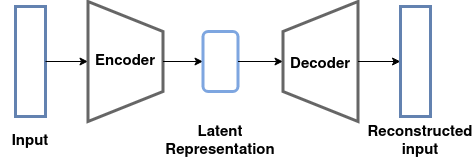
\includegraphics[width=0.75\textwidth]{AE_architecture}
    \caption{The architecture of an autoencoder.}
    \label{fig:AE_architecture}
\end{figure}

Formally, an autoencoder can be defined by the two functions it learns: 
\begin{equation}
  \label{enc}
  \phi :{\mathbb{R}^n}\rightarrow {\mathbb{R}^m}
\end{equation}
\begin{equation}
  \label{dec}
  \psi :{\mathbb{R}^m}\rightarrow {\mathbb{R}^n}
\end{equation}
\begin{equation}
  \label{encdec}
  \phi ,\psi ={\underset {\phi ,\psi }{\operatorname {arg\,min} }}\,{\Delta}(x, \psi \circ \phi (x))
\end{equation}
Equation~\eqref{enc} defines the encoder and equation~\eqref{dec} the decoder, both satisfying~\eqref{encdec} where $\Delta$ is the reconstruction loss function for input x. The closer the output of the autoencoder approximates the original input, the lower the loss.

A fundamental difference with using PCA, is the type of functions that can be approximated for lowering the dimensionality. Since an autoencoder uses neural networks, they can approximate nonlinear functions, as mentioned in section \ref{pl-nn}. This is in contrast with PCA, which can only approximate linear functions. Because of this, an autoencoder can learn more powerful generalisations which leads to lower information loss\cite{AE_general}.

To use an autoencoder for state-space dimensionality reduction, we again (like with PCA) use as input an observation the agent got from the environment. We can train the autoencoder using both the encoder and the decoder to calculate the loss. When used in RL, only the encoder is used. The encoder will project the observation input to the dimensionality of the latent space. 

\subsection{DeepMDP}\label{pl-deepmdp}
Info over deepmdp

\chapter{Research}\label{research}
%TODO Mention RQ, problem statement
The aim of this paper is to examine the effect of reducing the dimensionality of the state-space in reinforcement learning (RL). In this section we will discuss the our research and its results. We will start by detailing our method in section \ref{research-method}; here we will explain the environments we used for our experiments, as well as the experiments that we ran. After this, we will show and discuss the results from these experiments in section \ref{research-results}. The discussion of the results will include an examination of how the different state-space reduction methods led to their results.

\section{Method}\label{research-method}
In this section we will explain our method: how we researched the effect of state-space dimensionality reduction on an RL agent. First, in section \ref{research-exp}, we will explain the experiments in general: the different agent setups that we compared. Then, we will look at the environments in which we ran the experiments in sections \ref{research-env-pysc2} and \ref{research-env-pong}, including their specific agent architectures.

\subsection{Experiments}\label{research-exp}
To examine the effect of the different dimensionality reduction methods, we implemented multiple RL agents using different reduction methods and compared their performance in two environments. In this section we will discuss the agents that we used. We will give a general overview here, and give more details about the architectures of the agents in the sections explaining the used environments: sections \ref{research-env-pysc2} and \ref{research-env-pong}.

The first agent mentioned is the baseline agent, which does not use a dimensionality reduction method, therefore using the full dimensions of the observation received from the environment. All other agents reduce the dimensionality of the observations, thus using less features.

Furthermore, to allow for a fair comparison of their performance, all agents must share as many architectural design choices and hyperparameter settings as possible. This is done by extending the baseline agent in all other agents. 

\noindent \textbf{Baseline agent}\newline
\noindent The baseline agent is a standard RL agent that does not use any dimensionality reduction. This is the agent that is extended by all other agents. It uses a DDQN strategy, as explained in section \ref{pl-dqn}. 

First, the agent receives an observation from the environment. This observation is passed to its neural network approximating the Q-function: its policy network. This returns a valuation for each action taken in this state. Then, the agent either chooses the action with the best valuation (i.e. acting greedily) or chooses a random action. Then, the chosen action is performed and we repeat this cycle until the end of the episode, whilst often training the policy network on stored transitions.

\noindent \textbf{PCA agent}\newline
\noindent The PCA agent uses PCA to reduce the dimensionality of the state observations. As mentioned, this is done by extending the baseline agent: after receiving an observation from the environment, the observation is processed by a PCA component lowering the observation dimensionality. This latent representation is then used by the agent as if it is the actual observations. This means that it is passed to the policy network to give an action valuation, as well as being stored in transitions used to train the network.

The PCA component is trained separately before being used by the agent. This is done by training the PCA on previously stored observations. It is important that these observations give a good representation of the entire environment to get a well trained PCA component.

\noindent \textbf{Pre-trained autoencoder agent}\newline
\noindent This agent is very similar to the PCA agent, except instead of using a PCA component, we are using an autoencoder to reduce dimensionality. Just like the PCA component, the autoencoder is pre-trained on stored observations. After this it is used by the agent to reduce the dimensionality of the observation. 

The autoencoder is trained by passing batches of observations to the encoder, which performs the dimensionality reduction. Its output is then passed to the decoder which tries to reconstruct the original data. The loss is then calculated by how similar the decoder output is, compared to the original data. Specifically, the \emph{mean squared error} is used.

When being used by an agent to reduce the dimensionality of an observation, only the encoder part of the autoencoder is used. When we speak of the output of the autoencoder in the context of being used by an agent, we mean the output of the encoder part. The autoencoder is not being trained further while in use by an agent. \newline

\noindent \textbf{\todo{I guess "online" is not strictly correct}Online trained autoencoder agent}\newline
\noindent  This agent is very similar to the pre-trained autoencoder agent. The only difference is the moment of training the autoencoder. In the pre-trained autoencoder agent, the autoencoder is trained before being used by an agent, using previously stored observations. In this online trained autoencoder agent, we are using an autoencoder that has not been pre-trained; it is being trained while being used by the agent. 

In this case, the agent itself still only uses the encoder part of the autoencoder. However, we now also store batches of observations and pass these to the training method of the autoencoder. This training method is the same as before: passing the observations to the encoder, whose output is passed to the decoder, whose output is compared to the original observation to calculate the loss and train the network.\newline

\noindent \textbf{DeepMDP agent}\newline
\noindent Just like the online trained autoencoder agent, the DeepMDP agent is completely trained while being used by the agent. It also uses an encoder, which has the same design as the encoders of the autoencoders. Differently from the autoencoder though, this encoder is actually part of the agent's network; whereas the autoencoder is a separate network, the DeepMDP simply extends the network of the agent, thus training the policy network and encoder simultaneously. This is further explained in section \ref{pl-deepmdp}.

In figure ... it can be seen that the observation given by the environment goes directly into the policy network. However, in contrast with the baseline agent, the observation first goes through the encoder, before going into the network representing the Q-function.

Another difference with the baseline agent is not shown in the figure: the DeepMDP makes use of an auxiliary objective to calculate the loss while training the policy network: the transition loss. This is also explained in section \ref{pl-deepmdp}.

\subsection{Environment: Starcraft II}\label{research-env-pysc2}
For our experiments we used the \emph{StarCraft II} environment by \emph{Blizzard}\cite{blizzard}. StarCraft II is a real-time strategy game, which has been used in RL research after the introduction of a learning environment created in collaboration with \emph{DeepMind}, called \emph{SC2LE} and a corresponding Python component called \emph{PySC2}\cite{pysc2}.

In particular we are using a PySC2 minigame called \emph{MoveToBeacon}. This minigame simplifies the StarCraft II game. Here, the RL agent must select an army unit and move it to a given beacon. To simplify our RL agent, selecting the army unit is implemented as a script, thereby focusing our research on moving the army unit to the beacon. A screenshot of the game is given in figure \ref{fig:pysc2_SS}. 

\begin{figure}[h]
    \centering
    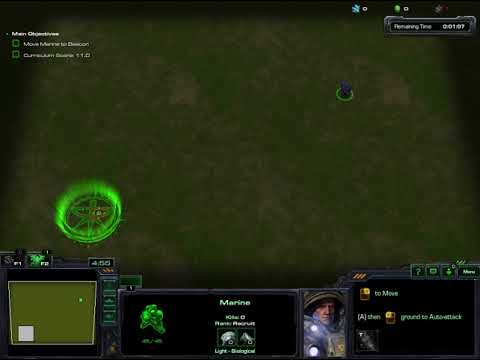
\includegraphics[width=0.75\textwidth]{pysc2_SS}
    \caption{Screenshot of the minigame \emph{MoveToBeacon} in \emph{StarCraft II}.}
    \label{fig:pysc2_SS}
\end{figure}

An \textbf{observation} received by the agent in this minigame is given by a $32 \times 32$ grid, representing the entire state of the game, \todo{Is this correct? Or are there actually perhaps only 3 features or something?} giving a total of \textbf{$1024$ features}. Each cell in the grid represents a tile in the game. It can have one of three values: a 0 denoting an empty tile, a 1 denoting the army unit controlled by the agent, or a 5 denoting the beacon. The beacon comprises more than one tile, namely a total of $21$ tiles; it comprises five adjecent rows, where the first comprises three adjecent columns, followed by three rows of five columns, followed by a row of three columns. Because of this, the beacon has $27 \cdot 27$ places where it could be, with the army unit having $1003$ tiles left to be. This gives \todo{Is this a correct usage of state-space?} a total state-space of $32 \times 32$ with a cardinality of $27 \cdot 27 \cdot 1003 = 731.187$. An example of such a state observation can be seen in figure \ref{fig:state_example}.

\begin{figure}[h]
    \centering
    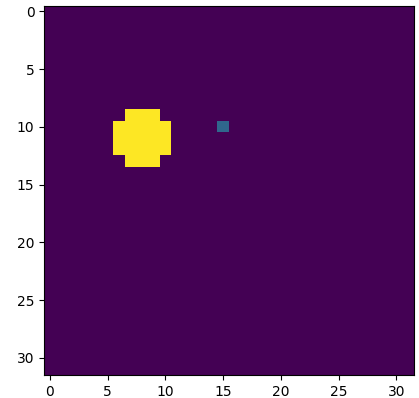
\includegraphics[width=0.75\textwidth]{AE_State_original}
    \caption{A state observation received by the RL agent, for the StarCraft II minigame MoveToBeacon. The yellow cells represent one beacon; the blue cell represents the army unit controlled by the player; all other cells are empty.}
    \label{fig:state_example}
\end{figure}

An \textbf{action} taken by the agent is given by an $(x,y)$ coordinate with $x,y \in \{0 .. 31\}$. This denotes the (indices of the) cell in the grid that the army unit will move to. Each action sent to the environment will result in $8$ in-game steps, meaning that if the given coordinates are further away than 8 steps, the unit will only walk 8 steps towards the given coordinates before the agent has to choose a new action.

Lastly, an \textbf{episode} takes $120$ seconds. The goal is to move the army unit to the beacon as often as possible in this time limit, each time adding $1$ point to the episode score. At the start of each episode, the beacon and army unit are placed randomly. Whenever the army unit reaches the beacon, only the beacon will be relocated randomly. 

Within the $120$s time limit, the agent will be able to take 239 steps/actions. An agent following a random policy gets a score of about $0-3$ points per episode (again, one point for each time the army unit reaches the beacon), whereas a scripted agent scores about $25-30$ points per episode (meaning the agent on average needs $8$ or $9$ actions before reaching a beacon).

\subsubsection{Agents setup}
We will now explain the architectures of the agents used in the Starcraft II environment. We will only give a general overview, referring to appendix \ref{appendix} section \ref{appendix-agents} for details on the neural network architectures and hyperparameter settings. 

Whereas the baseline agent uses the $32 \times 32$ observations given by the environment, all other agents reduce the dimensionality to $16 \times 16$. This means that the number of features in an observation are reduced from \todo{Again, is this correct?}$1024$ to $256$.

Though the baseline agent's architecture is extended by all other agents (in order to keep the agents as similar as possible), one important change must be made. The policy networks of all agents are convolutional neural networks, and the output dimensions of a convolutional layer depends on the dimensions of its input. The baseline agent's policy network receives a $32 \times 32$ input, whereas the other agents receive a $16 \times 16$ input. In all cases, the output dimensions must be $32 \times 32$. This is because the network approximates the Q-function: a valuation of all actions for a given state. Since an action in our environment is defined by the coordinates the army unit must walk to, there are $32 \times 32$ possible actions. To deal with this difference in input dimensions, the first layer of the policy networks of the non-baseline agents are modified (using different stride and padding sizes) to increase the dimensionality to $32 \times 32$.\newline

\noindent \textbf{Baseline agent}\newline
\noindent The baseline agent is a standard RL agent that does not use any dimensionality reduction and is extended by the other agents.

Its policy network consists of three convolutional layers: the first layer being a transposed convolutional layer \cite{transpose}, the other two being regular convolutional layers. The use of the transposed convolutional layer allows for the possibility of upsampling the dimensionality of the given input. This is needed in agents using dimensionality reduction, where the input for the network is $16 \times 16$, but the output needs to be $32 \times 32$ to cover the action space. However, for our baseline agent, the input dimensions, $32 \times 32$, must remain the same, which is achieved by setting the stride of the first layer to $1$. This way, both the dimensions of the input and the output of the network are $32 \times 32$ (where its input represents the current state observation and its output the action valuation).\newline

\noindent \textbf{PCA agent}\newline
\noindent The PCA agent uses PCA to reduce the dimensionality of the state observations from $32 \times 32$ to $16 \times 16$. To do this, the observation input must first be flattened, and its output must be reshaped to $16 \times 16$.

The output of the policy network representing the Q-function must remain $32 \times 32$, since we have $32 \cdot 32$ possible actions: one action per coordinate. Therefore, the first layer in the policy network, the aforementioned transposed convolutional layer, has a stride of $2$ and an output padding of $1$. This changes the dimensions from $16 \times 16$ to $32 \times 32$. 

The PCA component is trained on $240.000$ previously stored observations, which corresponds to observations from $1000$ episodes. These have been gathered using a scripted agent. The first $256$ principal components in our PCA (representing a $16 \times 16$ dimensional observation), contain roughly $96\%$ of the variance of the original data. We are using a scalar to standardize the observation data as explained in section \ref{pl-pca}. \newline

\noindent \textbf{Pre-trained autoencoder agent}\newline
\noindent Just like the PCA component, the autoencoder is pre-trained on the same $240.000$ observations. After this its encoder is used by the agent to reduce the dimensionality of the observation. 

The encoder and decoder of the autoencoder are convolutional neural networks. The encoder uses two convolutional layers: the first has a stride of $2$, which reduces the dimension to $16 \times 16$. The decoder, which tries to reconstruct the original data, uses three convolutional layers. The first layer is a transposed convolutional layer with a stride of $2$, to bring the dimensions back to $32 \times 32$. The other two layers are regular convolutional layers. 
 
\noindent \textbf{\todo{I guess "online" is not strictly correct}Online trained autoencoder agent}\newline
\noindent  This agent has the exact same design as the pre-trained autoencoder agent. As mentioned, the only difference is the moment of training the autoencoder: instead of training on previously stored observations, we are now training the autoencoder simultaneously with the RL agent.

\noindent \textbf{DeepMDP agent}\newline
\noindent The encoder of the DeepMDP has the same design as the encoders of the autoencoders: one convolutional layer with stride $2$ to reduce dimensions and a second convolutional layer with stride $1$. 

The auxiliary objective to calculate the transition loss represents the cost of all possible transitions from a given latent representation. This means that its output has dimensions $(32 \times 32) \times 16 \times 16$. The tuple $(32, 32)$ represents the actions that can be taken in the current state, while the other two dimensions, $16 \times 16$ represent the next (predicted) latent observation. It has only one layer, a convolutional layer, with $32 \times 32$ output channels to represent the action dimensions.

\section{Results}\label{research-results}
In this section we will show and discuss the results from the experiments mentioned in section \ref{research-exp}. We start by discussing the general results of the agents in section \ref{research-general-results}, and then discussing and interpreting these results in section \ref{research-discussion}.

\subsection{Research results}\label{research-general-results}
The results from running the different agents in the Starcraft II minigame MoveToBeacon, can be seen in figure \ref{fig:results-agents}. For each agent, the score, i.e. reward, per episode is shown, as well as an average score per $30$ episodes. Again, a scripted agents scores around $25-30$ per episode, and an agent following a random policy around $0-3$.


\begin{figure}[h]
	\centering
	\begin{subfigure}[b]{0.75\textwidth}
		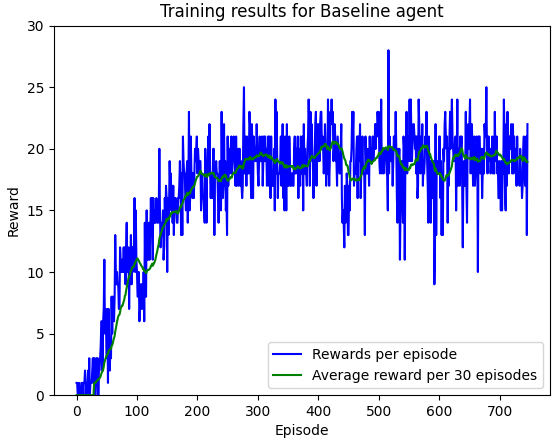
\includegraphics[width=0.75\linewidth]{Base_agent_results}
		\caption{Results for the baseline agent.}
		\label{fig:results-base} 
	\end{subfigure}
	\begin{subfigure}[b]{0.75\textwidth}
		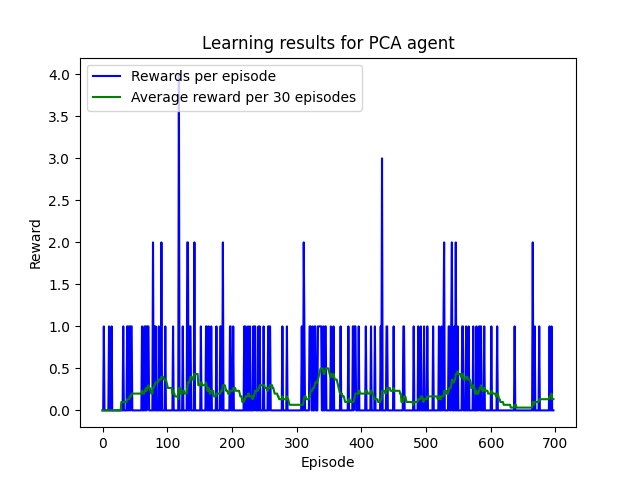
\includegraphics[width=0.75\linewidth]{PCA_with_scalar_agent_results}
		\caption{Results for the PCA agent using a scalar.}
		\label{fig:results-pca}
	\end{subfigure}
	\begin{subfigure}[b]{0.75\textwidth}
		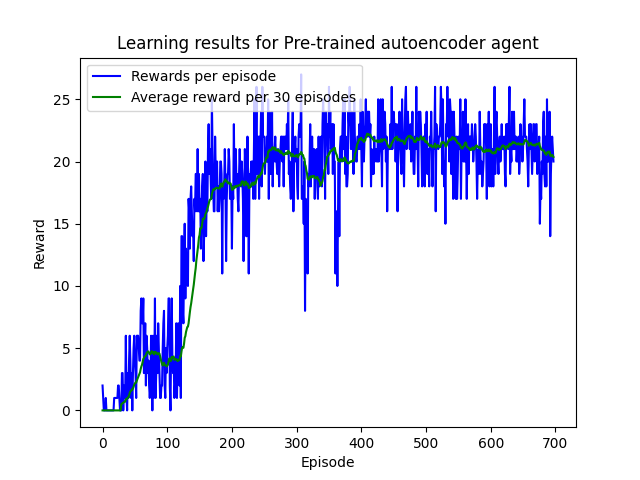
\includegraphics[width=0.75\linewidth]{Pretrained_autoencoder_agent_results}
		\caption{Results for the pre-trained autoencoder agent.}
		\label{fig:results-ae}
	\end{subfigure}
	\caption{Results of the different RL agents.}
\end{figure}%	
\begin{figure}[ht]\ContinuedFloat
	\begin{subfigure}[b]{0.75\textwidth}
		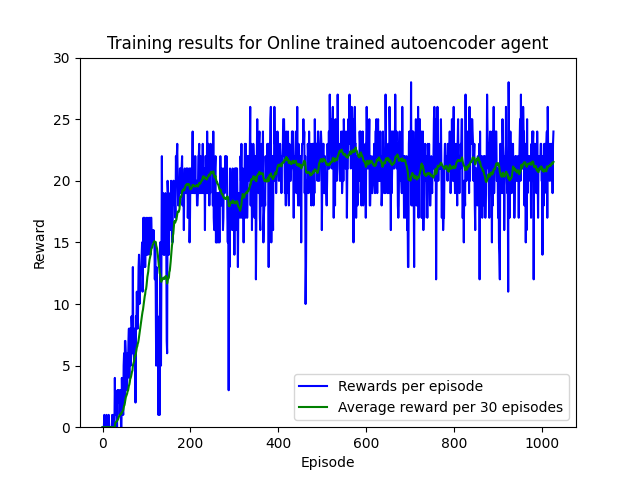
\includegraphics[width=0.75\linewidth]{Online_autoencoder_agent_results}
		\caption{Results for the online trained autoencoder agent.}
		\label{fig:results-online-ae}
	\end{subfigure}
	\begin{subfigure}[b]{0.75\textwidth}
		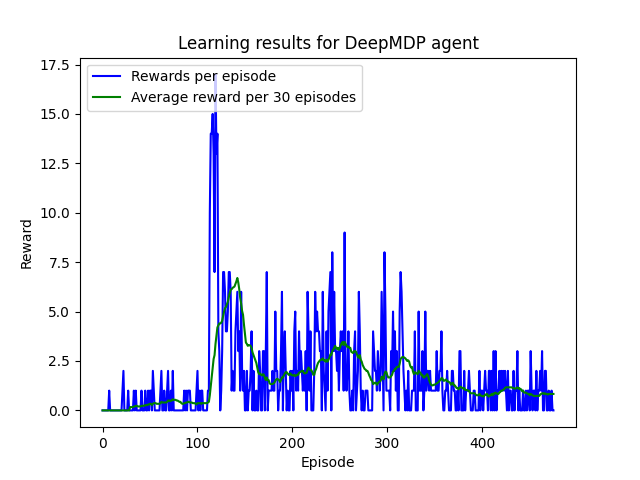
\includegraphics[width=0.75\linewidth]{Deepmdp_agent_results}
		\caption{Results for the DeepMDP agent.}
		\label{fig:results-deepmdp}
	\end{subfigure}
	\caption{Results of the different RL agents(cont.).}
	\label{fig:results-agents}
\end{figure}

As can be seen in subfigure \ref{fig:results-base}, the baseline agent converges to a policy scoring around $19$ per episode. This policy is reached after roughly $600$ episodes. Already after episode $300$ does it oscillate around scoring $17-20$ while also sometimes having an episode score of around $10$. After this it still needs another $300$ episodes to get to a more consistent policy.

The results for the PCA agent can be seen in figure \ref{fig:results-pca}. Though this shows the results for the agent using a PCA with a scalar, similar results were achieved without using a scalar. Furthermore, no matter what neural network architecture used in the agent (having used multiple different linear network architectures and different CNN architectures), it always remained at a policy performing at the level of a random policy, i.e. scoring around $0-3$ per episode.

The results for the agent using a pre-trained autoencoder, in figure \ref{fig:results-ae}, show that this agent preforms a little better. Not only does it converge to a slightly better policy scoring around $21$ per episode, it also converges quicker; it is already consistent after roughly $400$ episode, instead of $600$. 

We also show the results of training the autoencoder itself. As mentioned, it is trained on $240.000$ observations, corresponding to $1000$ episodes. Whereas each agent's training (except for the DeepMDP) took roughly $90$ minutes, training the autoencoder itself on $1000$ episodes worth of observations only took about $2.5$ minutes. The loss history for the autoencoder can be seen in figure \ref{fig:ae-loss}. After roughly $6000 \cdot 25 = 150.000$ observation it converges to its final loss.

\begin{figure}[h]
    \centering
    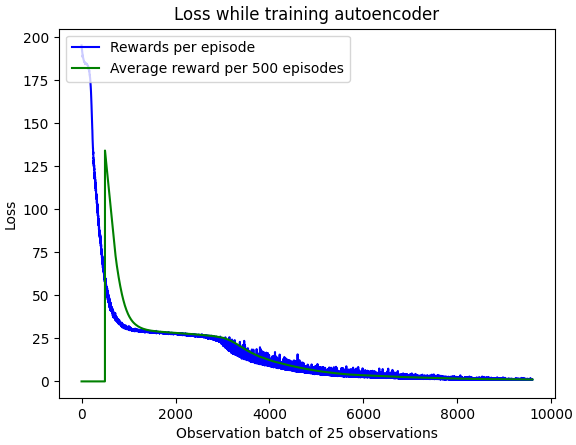
\includegraphics[width=1\textwidth]{ae_loss}
    \caption{Losses per 25 observations for training the autoencoder on $240.000$ state observations.}
    \label{fig:ae-loss}
\end{figure}

Compared to the pre-trained autoencoder agent, the agent using an untrained autoencoder that is being trained while the agent is trained, performs a little worse. It converges after roughly $500$ episodes to a policy around $19-21$. Not only does it take longer to converge and converges to a slightly worse policy, it is also less consistent. Even after $400$ it still has episodes scoring around $13$. This shows it is less consistent than its pre-trained counterpart.

Lastly we have the DeepMDP agent. After $130$ episodes, this agent suddenly jumps up from a random policy to scoring around $15$. However, after several episodes it starts going back down, alternating between scoring at a random policy and scoring around $7$, until finally reaching a random policy again. Furthermore it takes a lot longer to train. For the other agents, each episode took only a few seconds, whereas each episode in the DeepMDP agent takes $2.5$ minutes.

\subsection{Discussion}\label{research-discussion}
The first notable results is the PCA agent giving a policy that remains at a policy at the level of a random policy during its $800$ episode training, therewith performing way worse than the other agents. A possible explanation might be that the PCA reduction loses (too much) spatial information. \todo{Citing}Although PCA can be used for image compression, where spatial information is retained, it is a lot more lossy than for instance an autoencoder.

Figure \ref{fig:pca-state} shows an example of the PCA transformation on an observation. figure \ref{fig:pca-original} shows the original observation that the agent would get from the environment. Figure \ref{fig:pca-latent} shows the latent representation after using PCA for dimensionality reduction. as mentioned before, this uses $256$ principal components, capturing roughly $96\%$ of the original data. Here we can see that no spatial information is retained, making it impossible for the agent to train a meaningful policy on. 

Furthermore, we also tested a different PCA setup where we used all $1024$ principal components. Here, we again fitted the PCA on the same observations but keeping all principal components, giving a new $32 \times 32$ observation (and therefore not doing any dimensionality reduction). Transformation of an observation gave similar results: spatial information was lost. The problem therefore lies in the fitting process. A possible explanation for the bad transformation performance, might be that a single observation is very sparse. Even though the PCA is fitted on $240.000$ observations, each single observation is very sparse and at the same time, there are a lot of different possible observations due to the large state-space (see section \ref{research-env}). This combination might lead to the PCA not being able to generalize well enough. 

\begin{figure}[h]
	\centering
	\begin{subfigure}[b]{0.75\textwidth}
		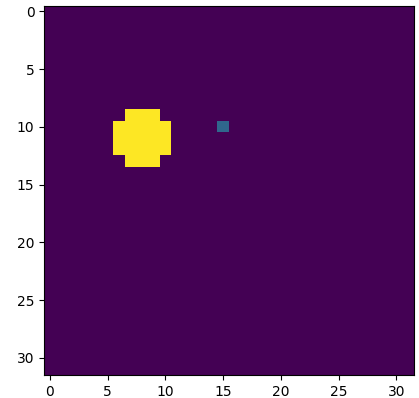
\includegraphics[width=0.75\linewidth]{AE_State_original}
		\caption{The original observation, i.e. the input for the PCA transformation.}
		\label{fig:pca-original} 
	\end{subfigure}
	\begin{subfigure}[b]{0.75\textwidth}
		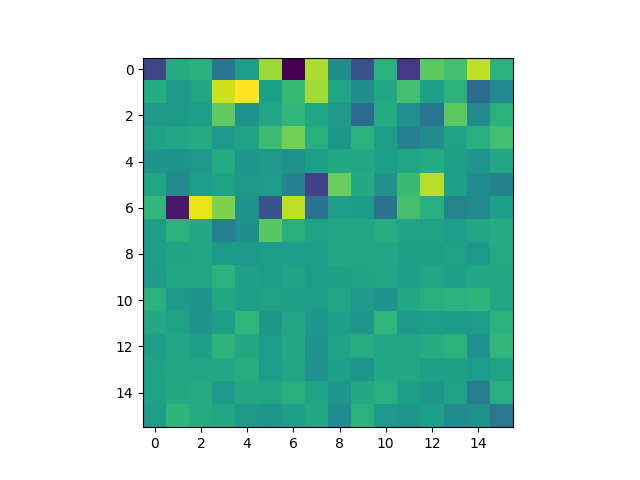
\includegraphics[width=0.75\linewidth]{pca_with_scalar_latent_state}
		\caption{The latent representation given by the PCA transformation}
		\label{fig:pca-latent}
	\end{subfigure}
	\caption{Latent representation and reconstruction of a state observation using PCA.}
	\label{fig:pca-state}
\end{figure}

Another interesting result is the performance of the pre-trained autoencoder agent. Not only does it match the baseline agent's performance, it even slightly surpasses it: it finds a slightly better policy (scoring around $21$ per episode on average, versus $19$), and more quickly converges to a consistent policy (after $400$ episodes versus $600$). Its better performance is despite the agent using imperfect information, while the baseline agent uses complete information.

Its performance is highly dependent on the quality of the output of the autoencoder. To get an understanding of why this agent achieves such good results, we will now examine the autoencoder in detail. Firstly, a correlation matrix is given in figure \ref{fig:ae-corr}. Based on $60.000$ state observations, it shows the correlation between the features of the original state observations (i.e. the input for the autoencoder) and the reduced state observations (i.e. the output of the autoencoder). The original data has dimensions of $32 \times 32$, whereas the reduced data has dimensions of $16 \times 16$, resulting in $1024$ and $246$ features respectively. Dark/black and light/beige colouring mean a high correlation (negative and positive correlation respectively), whereas a red colouring means no correlation and the white space means there was to too little variance to calculate a correlation. The latter case simply follows from the beacon and army unit not visiting these parts of the map enough times during the used episode observations.

What can be seen from this matrix, is that each cell in the reduced data grid, correlates to a block (a few adjacent rows and columns) of cells of the original data grid. This explanation can be abducted from each feature of the reduced data being highly correlated to a few features of the original data, then being uncorrelated for $32$ features, after which highly correlated features are found again. This jump of $32$ features corresponds to a jump of one row in the original data grid. Thus, a reduced feature correlates to a block of the original features.

\begin{figure}
	\centering
	\makebox[0pt]{%
	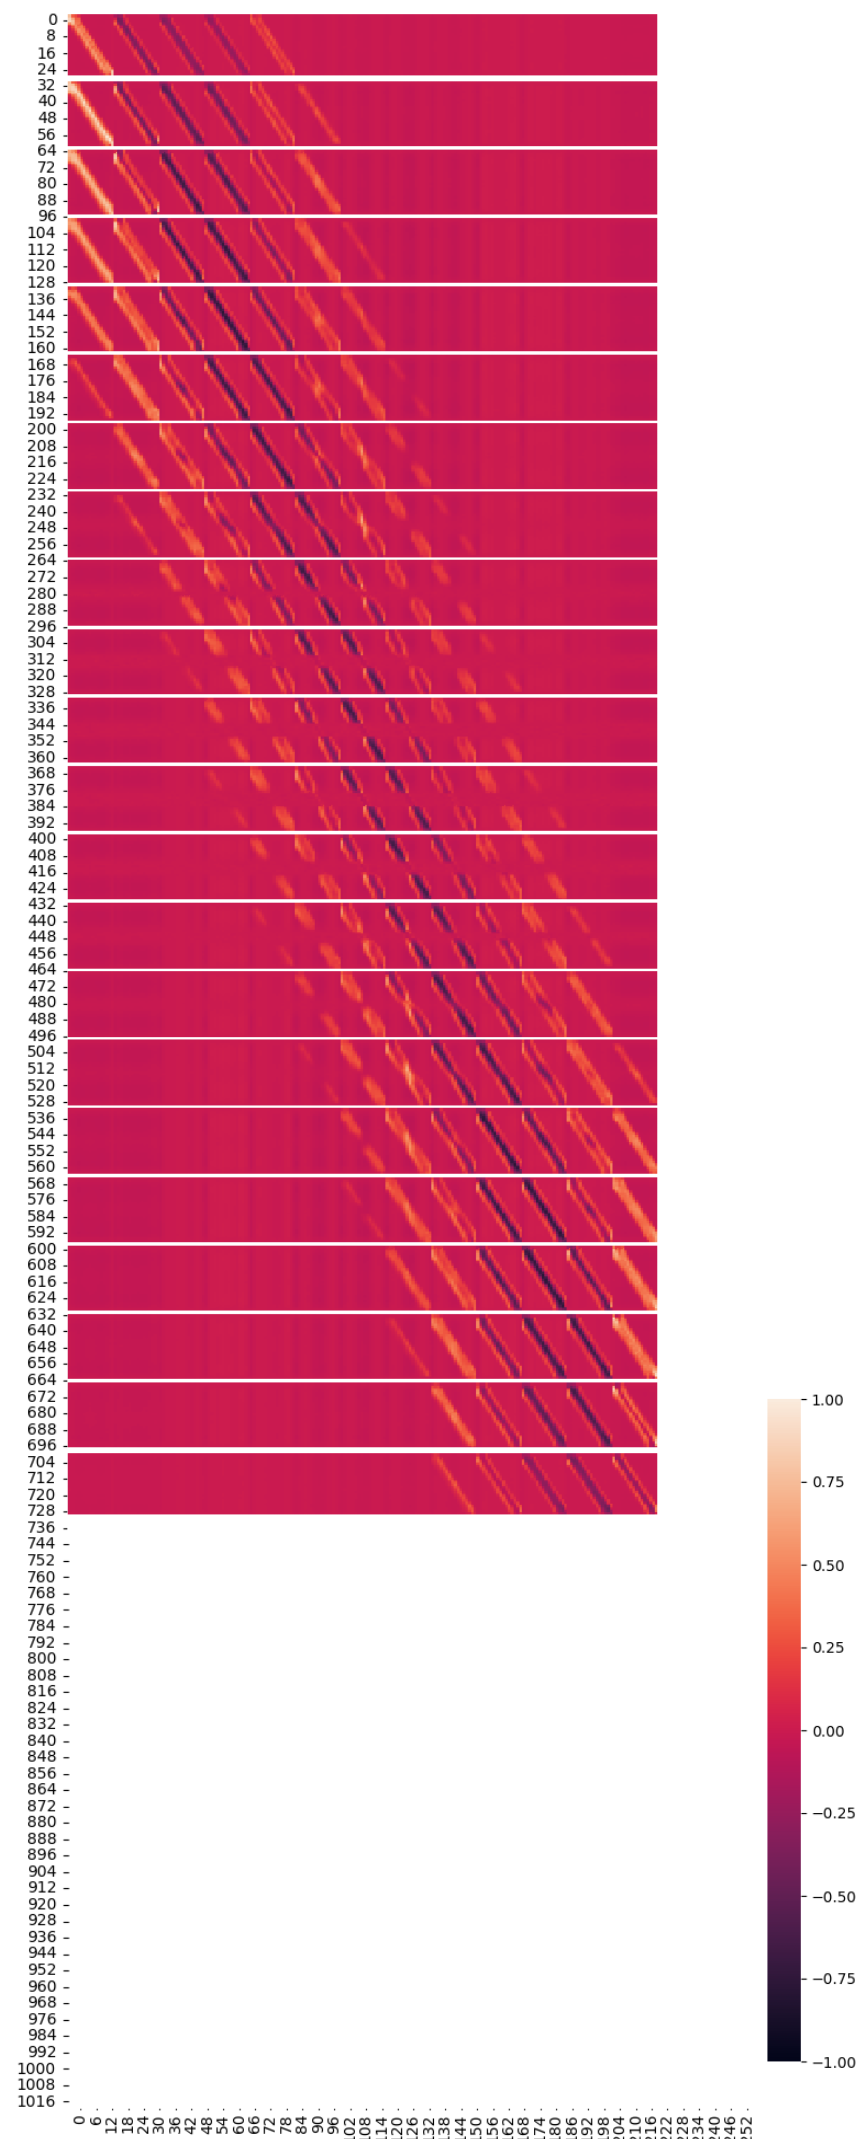
\includegraphics[width=1.0\paperwidth]{AE_corr_matrix_cropped}}
	\caption{Correlation matrix for the autoencoder used in the pre-trained autoencoder agent, based on $60.000$ state observations. The x-axis contains the features of the original observations, and the y-axis contains the features of the reduced state observations.}
	\label{fig:ae-corr}
\end{figure}

We also show the feature map visualisation for the enoder of the autoencoder in figure \ref{fig:ae-featuremap}. This shows the output of each channel in each convolutional layer of the encoder of the autoencoder. The original $32 \times 32$ input for the encoder is given in figure \ref{fig:ae-featuremap-original}. Like before, the yellow octagon is the beacon, the blue square is the army unit controlled by the agent, and purple parts are the empty tiles. The feature map for the first convolutional layer is given in figure \ref{fig:ae-featuremap-layer1}. It shows the output of its $32$ channels, each having a dimensionality of $16 \times 16$. What can be seen here is that each channel seems to pay attention to a different part of the observation, sometimes putting more emphasis on the empty cells, sometimes more on a certain side of the beacon and/or the army unit. Lastly the feature map of the second layer is given in figure \ref{fig:ae-featuremap-layer2}. Since this has only one channel, this also corresponds to the output of the encoder. 


\begin{figure}[h]
	\centering
	\begin{subfigure}[b]{1\textwidth}
		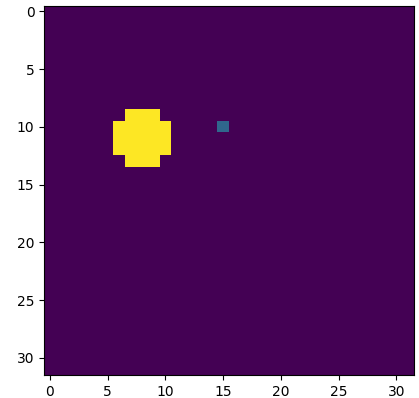
\includegraphics[width=1\linewidth]{AE_State_original}
		\caption{The original observation, i.e. the input for the autoencoder.}
		\label{fig:ae-featuremap-original} 
	\end{subfigure}
	\begin{subfigure}[b]{1\textwidth}
		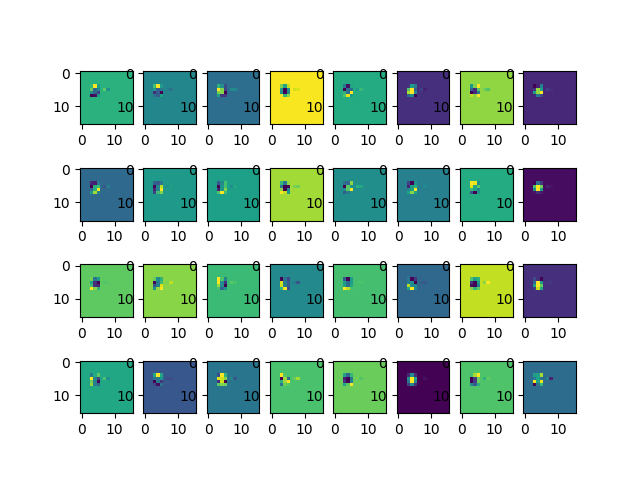
\includegraphics[width=1\linewidth]{AE_Layer_1_Feature_Map}
		\caption{The feauture map of the first convoluational layer, showing the output of its $32$ channels.}
		\label{fig:ae-featuremap-layer1}
	\end{subfigure}
	\caption{A feature map visualisation for the autoencoder used by the pre-trained autoencoder agent.}
\end{figure}%	
\begin{figure}[ht]\ContinuedFloat
	\begin{subfigure}[b]{1\textwidth}
		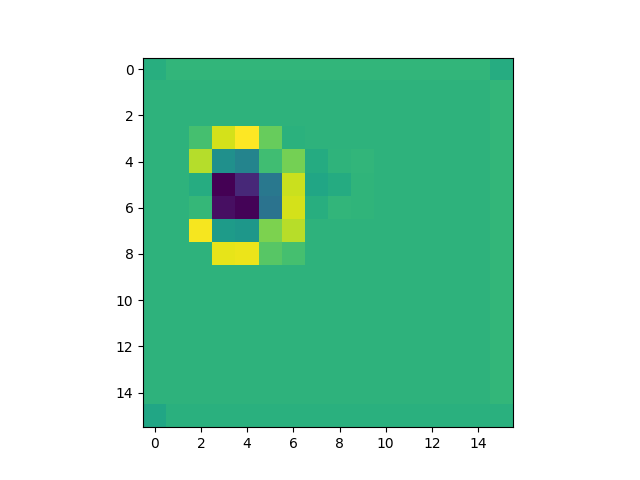
\includegraphics[width=1\linewidth]{AE_Layer_2_Feature_Map}
		\caption{The feature map of the second convolutional layer, showing the output of its single channel. Since it has only one channel, this also corresponds to the output of the autoencoder.}
		\label{fig:ae-featuremap-layer2}
	\end{subfigure}
	\caption{A feature map visualisation for the autoencoder used by the pre-trained autoencoder agent (cont.).}
	\label{fig:ae-featuremap}
\end{figure}

This autoencoder agent not only outperforms the baseline agent, it also (less surprisingly) outperforms the online trained autoencoder agent. This latter agent converges to a slightly worse policy and takes more episodes to get there, while remaining not very consistent (sometimes scoring only about $13$ points in an episode). This can of course be explained by the fact that this agent not only trains a policy network, but also, separately, the autoencoder. This means that for many episodes, the policy network is trained on a rather imperfect representation; the pre-trained autoencoder needed roughly $150.000$ observations before getting close to its final loss. Still, it got to a policy similar to the baseline agent (even scoring slightly better on average) in a similar number of episodes; the main difference being that the baseline agent is much more consistent. %TODO 180.000 beter bekijken, gegokt

Besides outperforming the online trained autoencoder agent, the pre-trained agent has another advantage. Since the autoencoder can be trained separately from the agent, we can reuse the autoencoder for different agents acting in the same environment. This allows for the possibility of training an autoencoder once, after which multiple agents can be trained on less features, allowing for less computation cost to train each agent. This is also substantiated by the autoencoder taking little time train.

Lastly, the DeepMDP performs horribly and something seems off with its implementation, since it goes to a decent policy scoring around $15$ per episode, then quickly dropping back to the level of a random policy. I'm not sure what is going wrong here. I did print out the loss during a few different moments in training. Its loss calculation consists of several different losses: firstly the usual DDQN loss calculated like in all other agents. Secondly, the loss of the auxiliary objective: the transition loss. Lastly we have the gradient penalty for each part of the network. All these losses are added together, with the sum of the gradient penalties being multiplied by $0.1$ (a hyperparameter).

After $133$ episodes, when the agent gets decent scores of around $15$ points per episode, the losses look as follows:
\begin{itemize}
\item DDQN Loss: 0.008
\item Transition Loss: 400
\item Encoder gradient penalty: 20
\item Policy gradient penalty: 20
\item Auxiliary objective gradient penalty: 3.5 million
\item Total loss: 38.000
\end{itemize}

A few episodes later, it goes down to a policy scoring about $0$ per episode:
\begin{itemize}
\item DDQN Loss: 0.002
\item Transition Loss: 1000
\item Encoder gradient penalty: 90
\item Policy gradient penalty: 90
\item Auxiliary objective gradient penalty: 1.5 million
\item Total loss: 16.000
\end{itemize}

After $248$ episodes, it is still at the level of a random policy:
\begin{itemize}
\item DDQN Loss: 0.0008 
\item Transition Loss: 22.000
\item Encoder gradient penalty: 3.5
\item Policy gradient penalty: 3.5
\item Auxiliary objective gradient penalty: 2000
\item Total loss: 22.000
\end{itemize}

We can see here that there is probably something off with the loss calculation, since they are extremely disproportional.
OR PERHAPS the problem lies in that there is no good prediction of transition (i.e. next state) possible due to the continuous random replacement of the beacon when following a good policy and therefore the only way to lower the transition loss (does this also entail the aux penalty?) would be to follow a policy that does not reach the beacon.
\chapter{Conclusions and future research}\label{conclusions}
In this thesis we compared multiple state-space dimensionality reduction methods for a model-free, value-based reinforcement learning (RL) agent, using two environments: Starcraft II MoveToBeacon and OpenAI Atari Pong. We tried to answer the research question: \textit{what is the effect of state-space dimensionality reduction on model-free value-based reinforcement learning in an environment using spatial grid-based observations, by using PCA, autoencoders or DeepMDPs}? To answer this, we answered the research sub-question: \textit{how do the training results of a double deep-Q-network reinforcement learning agent change when using PCA, autoencoders and DeepMDPs for state-space dimensionality reduction in Starcraft II MoveToBeacon and OpenAI Atari Pong}? 

The PCA component was trained on previously gathered observations. In both environments, the PCA was unable to retain spatial information, despite using between $96\%$ and $99\%$ of the variance of the original observation. After training it was used in an RL agent to project the observation to a latent space, used by the RL agent to train its policy. Due to the lack of spatial information, needed for both environments, the PCA agent was unable to train well. Thus, PCA seems only promising for environments using non-spatial observations, like in Curran et al. where their PCA agent worked better than a baseline agent \cite{mario}.

The DeepMDP used in Starcraft II was also unable to train well. This is due to its difficulty in balancing multiple loss calculations. The DeepMDP agent initially trained to a decent policy, but then dropped down to a worse policy, due to the loss balancing problem. This is a known problem for DeepMDPs \cite{deepmdp}.

Lastly, the autoencoder was able to learn a good latent representation of the observations in both environments, meaning it accurately captured the dynamics of the original state space in a smaller dimensionality. We used the autoencoder in two different agent types. The first is the pre-trained autoencoder that is trained on previously gathered observations, as with PCA. This agent outperformed the baseline agent in Starcraft II, reaching a better and more consistent policy in fewer episodes: its average return increased roughly $10\%$ using $400$ instead of $600$ episodes to converge. In Pong it trained slightly worse than the baseline agent (a $20\%$ performance decrease), but still found a good policy (scoring about $70\%$ compared to an optimal, scripted agent). Its lesser performance here is explained by detailed spatial information being lost in the latent space.

The second autoencoder agent is the online trained autoencoder agent. Here, the autoencoder is trained simultaneously with the RL agent; thus the autoencoder is trained while being used to project observations to a latent representation. These agents took a longer time to train to a good policy but eventually reached one similar to the pre-trained autoencoder agent. This can be explained by the RL agent initially training on bad latent representation due to a yet badly trained autoencoder.

This showed the promise of using autoencoders for state-space dimensionality reduction in model-free RL agents. This allows for training agents in high dimensional environments, by projecting the observations to a lower dimensional space through state representation learning. This may result in lowered training times, on less observations and episodes, using less computation cost. Such a reduction component can also be used in different RL agents running in the same environment, solving different problems using the same latent representation. This way the autoencoder only has to be trained once for the environment, before being beneficial for the training of different RL agents. It also showed the limit of using an autoencoder for state-space dimensionality reduction in environments where detailed spatial information is necessary for the RL agent, since some of this might get lost in an even slightly inaccurate latent representation from the autoencoder.

PCA and DeepMDP showed less promise in these environments. The PCA lost its spatial information, and may thus be more applicable for non-spatial environments. The DeepMDP had trouble balancing its loss and was therefore unreliable.\newline

\noindent\textbf{Future work}\newline
\noindent For future work we suggest several possibilities. Firstly, we could try to improve on the experiments in this thesis. In particular, we could try to use a more complex autoencoder architecture, that only downsamples its input to a lower dimensional space in later layers of its encoder network (instead of doing this in the first layer like in this research). This way spatial information might be retained better, possibly resulting in even better training results in environments like Pong where spatial details are important. Secondly, we might use environments with non-spatial information to be able to compare the reductions methods here, to see how well PCA and DeepMDPs perform. 

Furthermore, we could examine the advantages of dimensionality reduction, since in this thesis we only focused on the feasibility of such agents. Whereas in this thesis we kept each agent as similar as possible to the baseline agent, for future research we could try to optimize the dimensionality reduction agents to train on latent spaces and policy networks that are as small as possible without converging to sub-optimal policies. This way we could better see the training advantages of such agents, both in terms of number of episodes and in terms of real training time. We could also examine the possibility of re-using the same reduction component in the same environment solving different RL problems.

\bibliographystyle{plain}
\bibliography{bibliography}

\appendix
\chapter{Appendix}\label{appendix}
\section{RL agent architectures}\label{appendix-agents}
Here we will lay out the details of the architecture and hyperparameter settings that were used in each agent mentioned in section \ref{research-method}. We will start by showing the vanilla agent, which uses an architecture and hyperparameters that are shared by all agents. For all other agents, each extending this vanilla agent, we will only give the additional architecture and parameters.

- ook adam function en relu oid, referentie naar bijbehorende papers

\subsection{Vanilla agent}
Jaaa JAAAAA


\end{document}
